\chapter{Analysis}
Template article citation\cite{articleTemplate}\\
Template online citation\cite{onlineTemplate}\\
Template book citation with page range\cite[p.~442-444]{interactionDesign}

\section{Analysis Intro}
In this analysis, the focus will be on the investigation of the current issues with the fundamentals of musical education in elementary schools.\\
\\
Furthermore, current tools and technological inventions will be investigated to incorporate the same aspects to a final prototype.

\section{The impact of musical education}
Several studies have shown that different types of musical engagement in a variety of ways over a lifespan has an impact on several aspects of personal development. As concluded in the article "The power of music: Its impact on the intellectual, social and personal development of children and young people":\\

\begin{quote}
	\textit{"This overview provides a strong case for the benefits of active engagement with music throughout the lifespan"}\cite{powerOfMusic}\label{quote:powerOfMusic}.\\
\end{quote}

Linguistic abilities and musical training seem to be linked as shared brain mechanisms are used to process music and language. Precision in the perception of speech related contrasts in pitch patterns and other distinctive speech elements have been reported to be associated with musical ability\cite{languageSkills}.

A study focused on literary skills showed that a group of second grade students(n = 47) taking piano lessons over a 3-year period had significantly better vocabulary and verbal abilities than a group of control students(n = 57) that did not receive music lessons\cite{vocabularySkills}.

Some aspects of mathematical skills have also shown to be improved by musical training. For example the sub-division process required to read and play from music scores in order to play keep a rhythm\cite{powerOfMusic}.

Other abilities have also been reported to be affected by musical training such as creativity, social and personal development, physical development, health and wellbeing\cite{powerOfMusic}.\\

According to Deirdre Russel-Bowie there are 5 basic musical elements that should be learned to have a good understanding of music\cite{primaryArts}:\todo{Maybe start with this part, to introduce section, or maybe move to Jens' section}
\begin{itemize}\label{list:basicMusic}
	\item Duration
	\item Pitch
	\item Tone color
	\item Dynamics
	\item Structure
\end{itemize}

\section{Problem Area}

	\subsection{Initial Research}
	To narrow down the subject and get a better understanding of what the problem is and which target group to work with, the study plans for danish elementary schools from grade 1 through 6 was investigated.\\
	\\
	According to the study plan, the children is required to learn three basic teaching elements. Within these are musical performance, musical creation and musical understanding.
	
	\subsection*{Musical performance}
	Musical performace includes teachings about singing, movement and playing instruments. More specifically teaching the children about how to sing individually and in groups, as well as teaching them about different kinds of singing and songs. Furthermore, teaching the children about movement in a musical context, such as dancing and rythmic movement. Finally, being able to play the basics of different instruments, such as drums, guitar, piano or keyboard and different wind instruments.
	
	\subsection*{Musical Creation}
	Musical creation includes the teachings of different abilities in relation to create, alternate or improvise musical pieces. The children should be able to compose music with the ability to remember time and tempo when creating music. Furthermore, the children should be able to form and shape sound into something rythmic. Besides creating music, the children should also be able to change music with the help of adding sounds, or changing the pitch or pace of sound. Finally, the children should be able to improvise music without being given a specific assignment to follow.
	
	\subsection*{Musical Understanding}
	Musical understanding is, first of, to be able to express music in other forms than sound. For an example, they should be able to express themselves verbally about music and be able to draw music. The children should have knowledge about instruments, and the ability to differ the different instruments from their appearance as well as their sound. The children should be able recognize specific elements in a musical piece and identify them. Finally, they should have the knowledge of musical history, in relation to different music genre as well as music from different time periods.
	\\
	
	When the children get older, they will be introduced to digital tools and syntesizers to be used in the classroom. These tools indclude digital devices such as iPads, as well as software such as Garageband. On these devices, they are asked to compose a musical piece using the aforementioned knowledge.\\
	In the lower grades, the children are working more with analog instruments as well as singing to develop a musical foundation for their education.
	\\
\begin{itemize}
	\item[-] Based on interviews and observations done with teachers and students
	\item[-] Issues in a musical classroom
	\item[-] Current tools, methods and the issues which is currently utilizing these resources
	\item[-] Possible investigations done beforehand and their results	
\end{itemize}

\section{Target Group}

\begin{itemize}
	\item[-] Elementary school children (Grade 1,2,3,4,5,6)
	\item[-] Potentially the teachers as a sub target group?\todo{Maybe other way around?}
\end{itemize}

\section{Motivation theory}
\todo{Maybe a section on motivation}
\subsection{The element of Surprise}
Studies have shown that surprise and novelty integrated into music instruction, can encourage children's interest, make them curious and pay attention. Adding an element of mystery and surprise can make them

\section{Interactivity of music learning}	
	When trying to understand music in an interactive sense, one might look at another medium that incorporates interactivity: video games. In particular, one could look at interactive video games that focuses around playing or teaching music. Lily Gower and Janet McDowall made a study, in 2012, focusing on the educational qualities gotten from playing these interactive music video games\cite{interactiveMusicVideoGames}. The study aims to establish if interactive music video games have an educational value when integrated into the existing music education.\\
	
	The different games mentioned in the study, was Guitar hero (See \autoref{sec:guitarHero}), SingStar and Wii Music. What these games have in common is that they all use interactivity as a means to playing music, be it with a guitar shaped controller, a microphone or the Wii remote held like an instrument. These games try to emulate what it would \textit{feel like} to play a guitar, sing or play different instruments.\\
	
	The study interviewed two music teachers of different musical affinities, and 9 music students aged 11-14 (5 male and 4 female) from different socio-economic situations. The student participants came into the study with different levels of musical experience. The interviews were semi-structured of nature to allow some free flowing conversation. Interviews with the children participants revolved around their prior music backgrounds and past experiences with interactive music video games. The interviews with the teacher participants discussed their personal views and experiences with interactive music video games, like Guitar hero (\autoref{sec:guitarHero}), in relation to music education.\\
	
	Teacher two said during the interview that:
	\begin{quote}
		\textit{"...the whole debate about whether it’s music making, that’s a whole other debate, but whether it’s developing some across the board generic skills, I’d say yes."}\cite[p.~98]{interactiveMusicVideoGames}.\\
	\end{quote}
	Meaning a belief in interactive music video games giving the students some educational values in a more general music setting. In addition when asked about coordination benefits, Teacher two said the following:
	\begin{quote}
		\textit{"...To play at the higher levels of that game [Guitar Hero] requires very high level coordination skills and you’re coordinating visually with what you’re playing as an instrument. So it’s not so different I think physiologically from what a musician does anyway which is to respond to a conductor visually, respond to the music score visually, and then play accordingly to a set tempo, and timing is everything. So, the game is about scoring high scores all based on your capacity to play in time on the right note and what’s that sound like? Sounds like music playing to me."}\cite[p.~98]{interactiveMusicVideoGames}.\\
	\end{quote}
	Teacher two has a firm belief that Guitar hero specifically has a high coordination requirement, and thus to play at the higher difficulty levels of the game, you need good eye-hand coordination, which he thinks correlates in a physiological way directly to the way real music is played.
	\begin{comment}
	The role of music education can be defined as:\todo{Think about way to use these two quotes nicely.}
	\begin{quote}
		\textit{"Teaching children to love music"}\cite[p.~94]{interactiveMusicVideoGames}.\\
	\end{quote}
	
	\begin{quote}
		\textit{Other key factors in motivation theory that can be identified within good video games include curiosity and a sense of autonomy or control over the learning that is occurring}\cite[p.~92]{interactiveMusicVideoGames}.\\
	\end{quote}
	\end{comment}
	\subsection*{Sub conclusion}
		In conclusion, according to Lily Gower and Janet McDowall's study\cite{interactiveMusicVideoGames}, interactive music video games can most likely teach children about pitch and rhythm (See all five elements in \autoref{list:basicMusic}), and might broaden their musical preferences. Hence interactivity might improve the way music is learned, at least in children.\todo{Maybe reword last part}

\section{State of the art}\label{sec:sota}
	\subsection{Guitar hero}\label{sec:guitarHero}
		\begin{figure}[H]
			\centering
			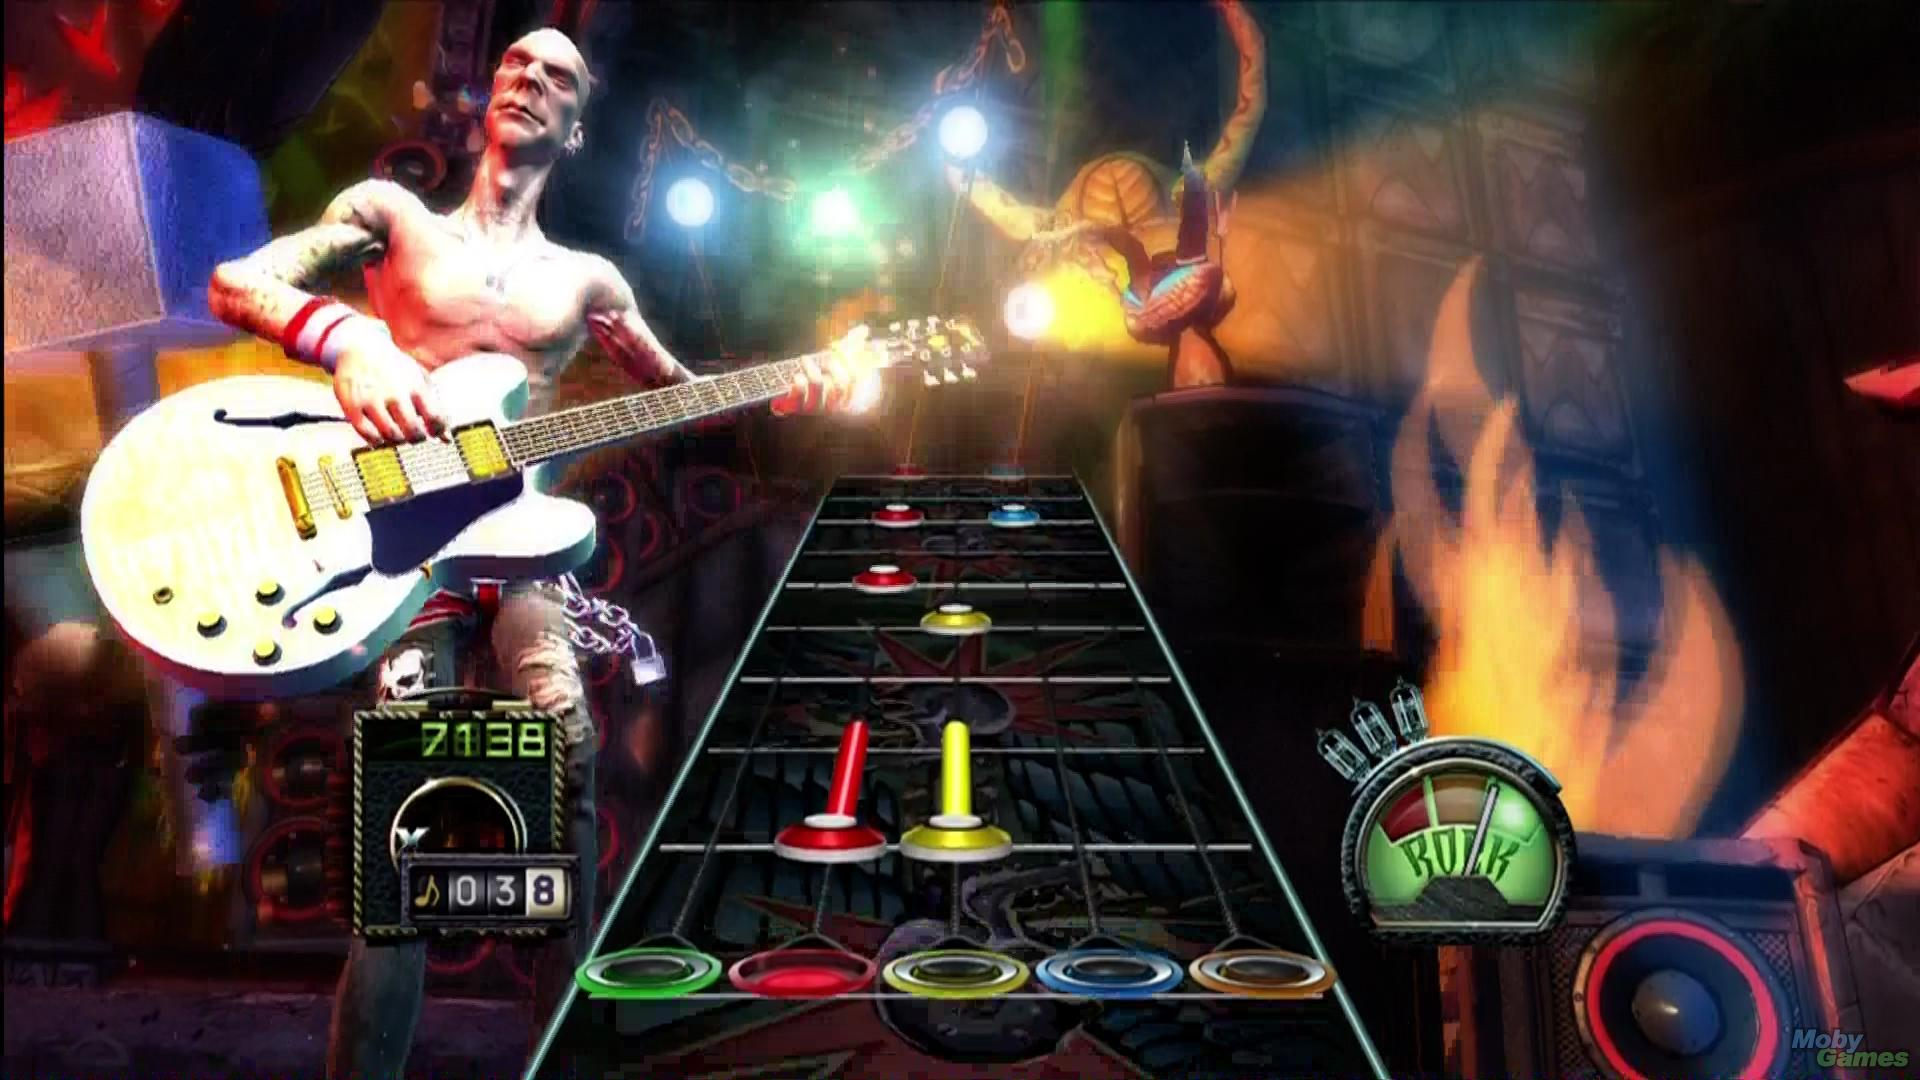
\includegraphics[width=0.7\linewidth]{figure/Analysis/guitarhero}
			\label{fig:guitarHero}
			\caption{Interactive music video game guitar hero.}
		\end{figure}
	\subsection{Noteput}
		German table where you physically put notes on it, and press play button to play notes, hopefully learning note and sheet theory.
	\subsection{Dato duo}
		Two person synthesizer for kids, to play around with, no apparent learning outcome, but seems fun to play around with.
		\begin{figure}[H]
			\centering
			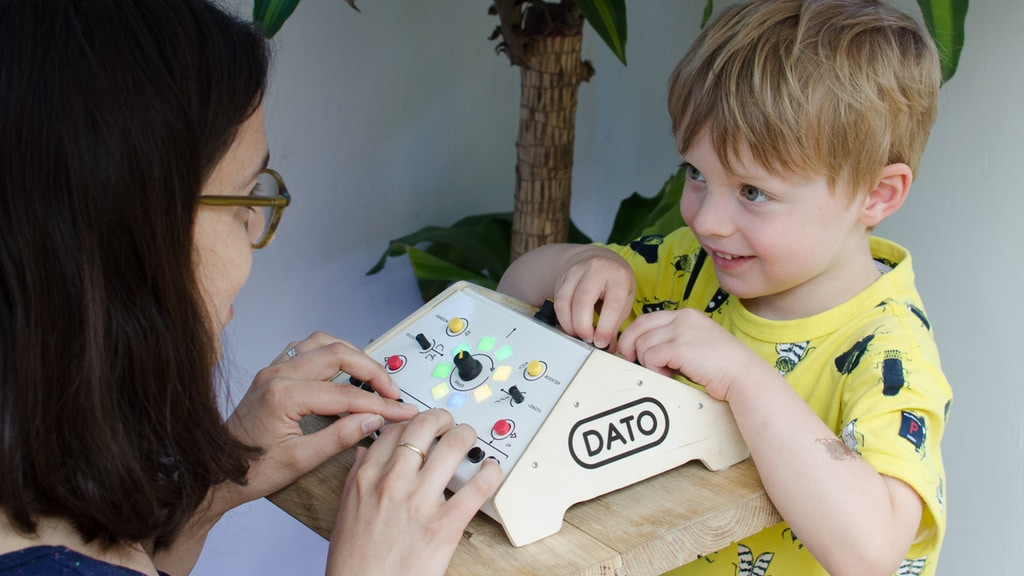
\includegraphics[width=0.7\linewidth]{figure/Analysis/datoduo}
			\label{fig:datoduo}
			\caption{Dato duo synthesizer}
		\end{figure}
	\subsection{Soundstage}
		VR application by Google, where you compose and play music in virtual reality. You can synthesize, plug things into other things, and create entire scores in this virtual reality playground.
		
	\subsection{V-Beat}
		The v-beat drumsticks are, for all its intents and purposes, simply air drumming.
		\begin{figure}[H]
			\centering
			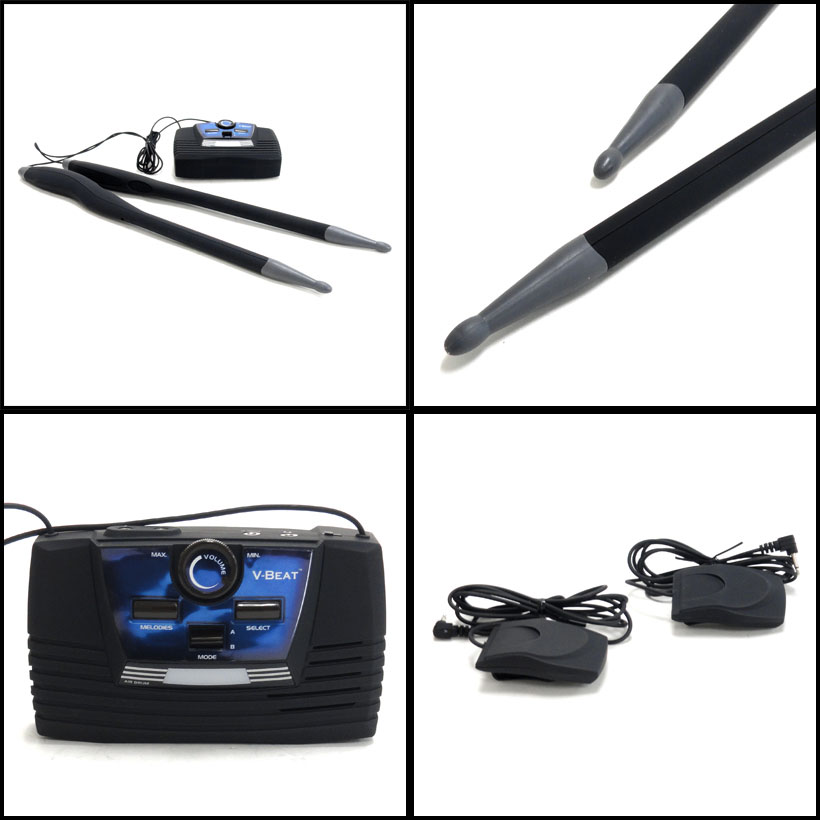
\includegraphics[width=0.5\linewidth]{figure/Analysis/vbeat}
			\label{fig:vbeat}
			\caption{Vbeat drumsticks}
		\end{figure}
		
	\subsection{MI Guitar}
		\begin{figure}[H]
			\centering
			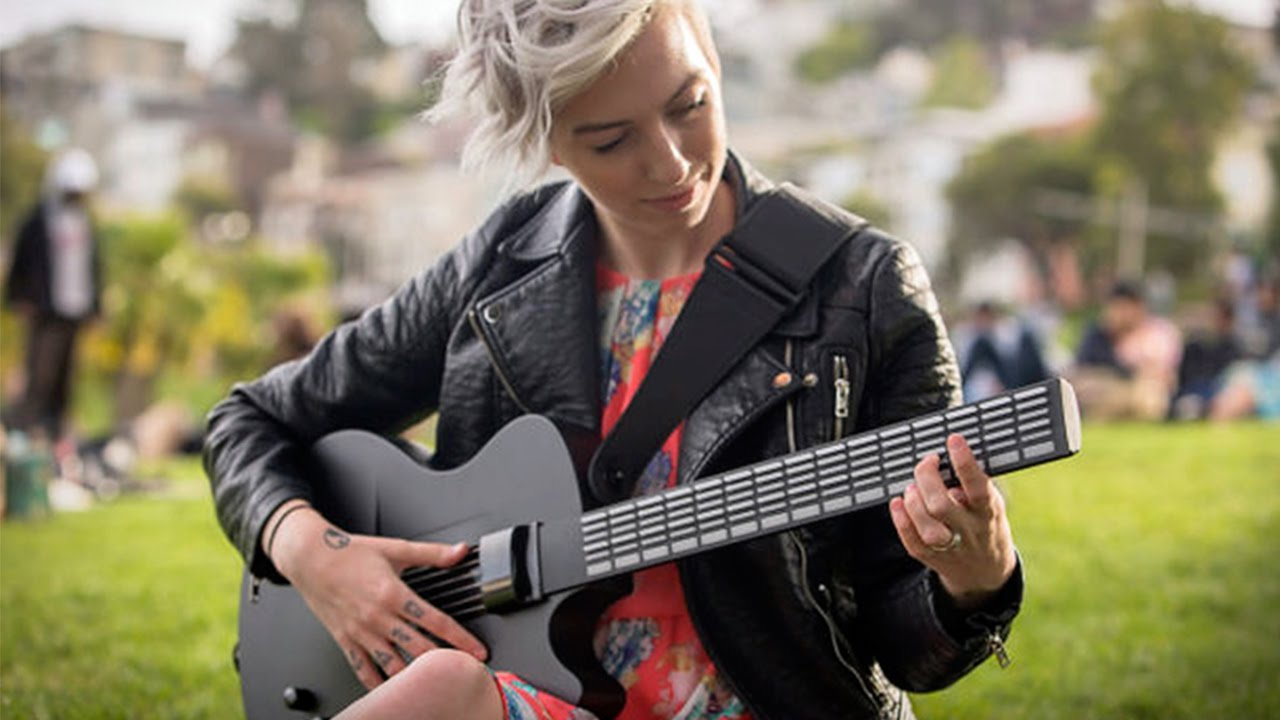
\includegraphics[width=0.8\linewidth]{figure/Analysis/miguitar}
			\label{fig:miguitar}
			\caption{MI guitar to teach guitar play}
		\end{figure}
	
	\subsection{Yousician}
		\begin{figure}[H]
			\centering
			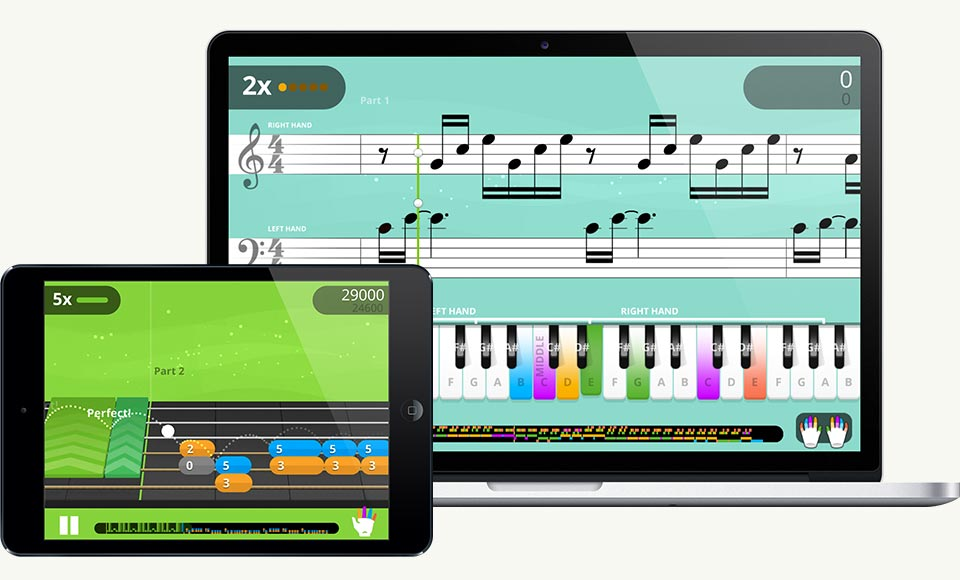
\includegraphics[width=0.8\linewidth]{figure/Analysis/yousician.jpg}
			\label{fig:yousician}
			\caption{Yousician}
		\end{figure}
	\subsection{Chrome Music Lab}
		\begin{figure}[H]
			\centering
			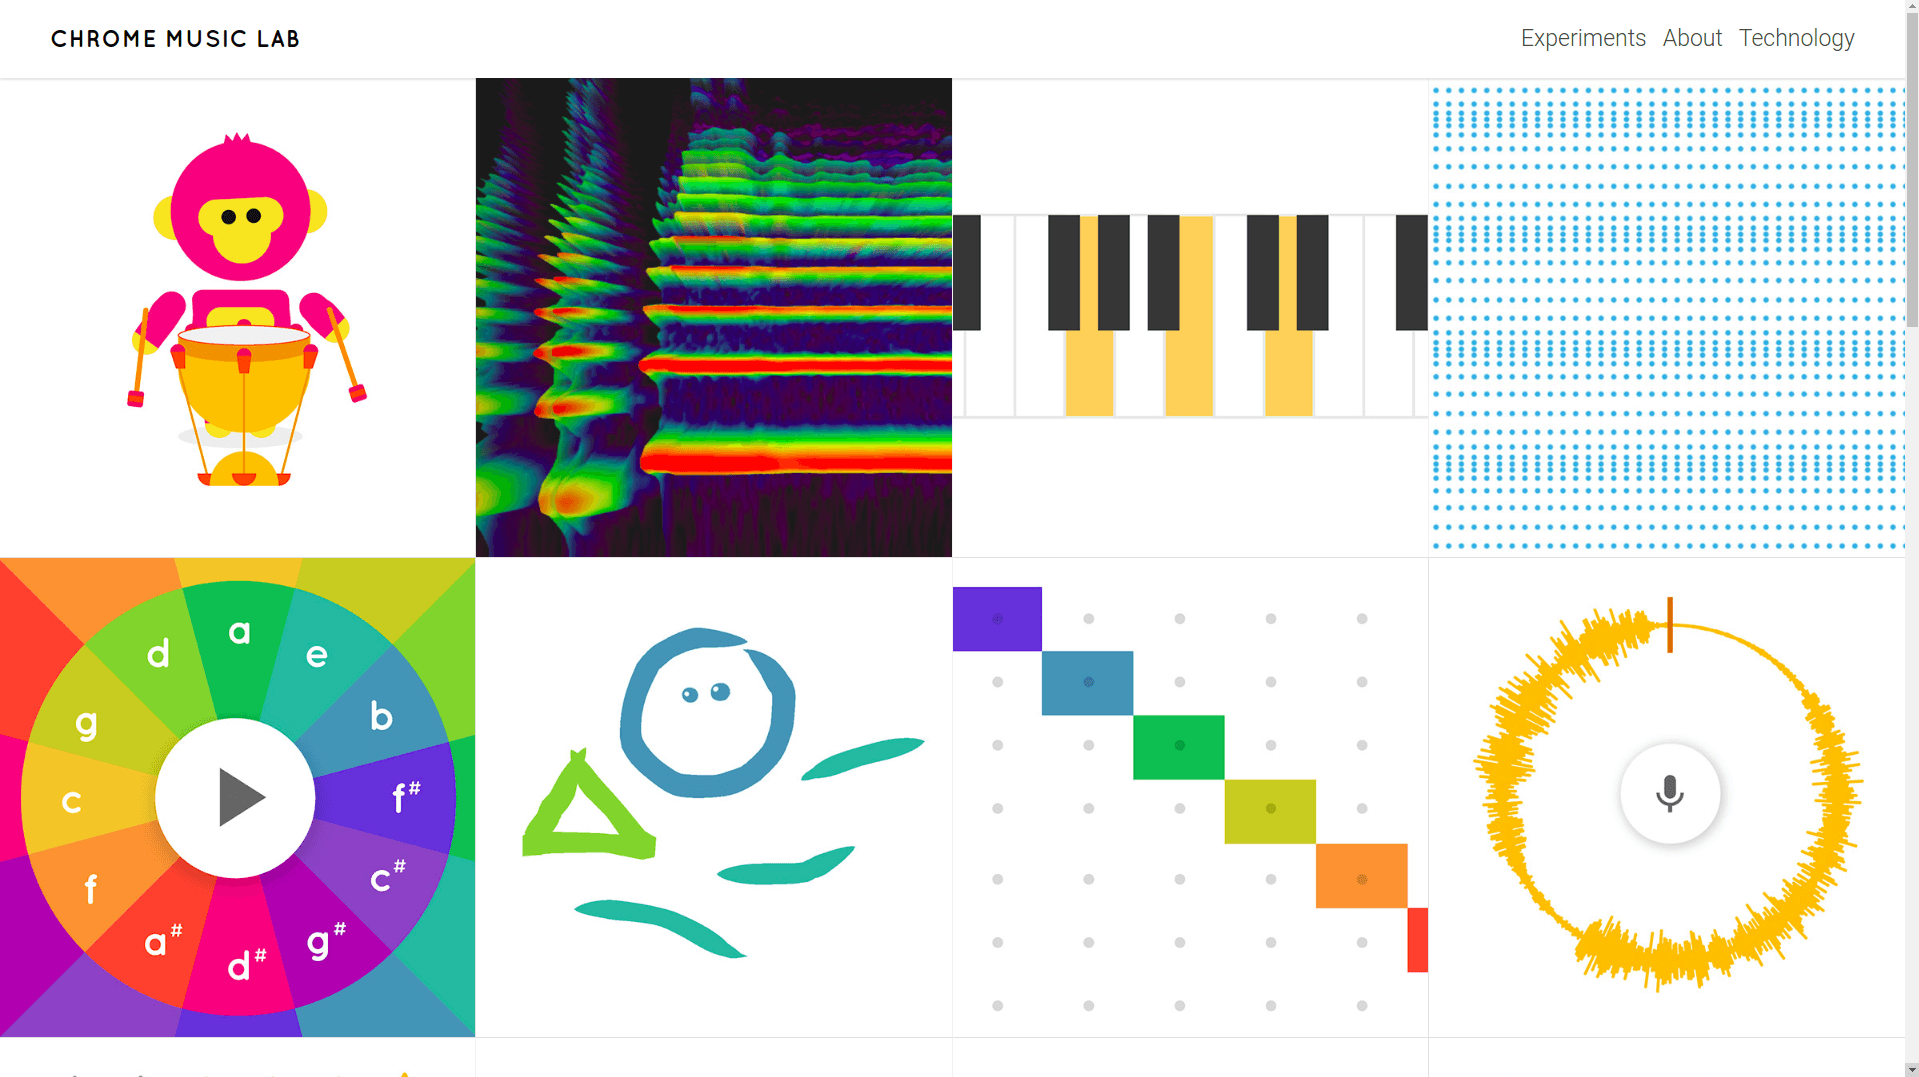
\includegraphics[width=0.8\linewidth]{figure/Analysis/chromeMusicLab.png}
			\label{fig:chromeMusicLab}
			\caption{Chrome Music Lab}
		\end{figure}

		